%\documentclass[10pt,a4paper]{report}
\documentclass[11pt,twoside,a4paper]{article}
\usepackage[utf8]{inputenc}
\usepackage{amsmath}
\usepackage{amsfonts}
\usepackage{amssymb}
\usepackage{graphicx}
\usepackage{caption}
\usepackage{subcaption}
\begin{document}
\begin{center}
Image Processing - Pattern recognition and drone controlling with OpenCV",
Gabriel Hidasy, Science without Borders - CAPES\\
Under supervision of Dr Adam Schiffer, University of Pécs - PMMIK\\
\today
\end{center}

\section{The Problem}
\paragraph {} In the context of this project a drone is an unmanned aerial
vehicle, capable of hover, particularly a Quad-copter.
\paragraph {} Drones can be controlled remotely by a human or by an autonomous
program,this project aims to produce a framework for controlling the drone from
a computer and integrate it with a pattern recognition algorithm to follow the
pattern in a room. This project does not aim to guarantee an stable flight
but the modular nature of it makes it easy to integrate it in another program.

\section{The equipment}
\paragraph {} The quad-copter used in this project is a Parrot AR-Drone 2.0, the
drone has a front facing camera and is controlled by WiFi.
\begin{figure}[hbtp]
  \centering
\begin{subfigure}{.99\textwidth}
  \centering
  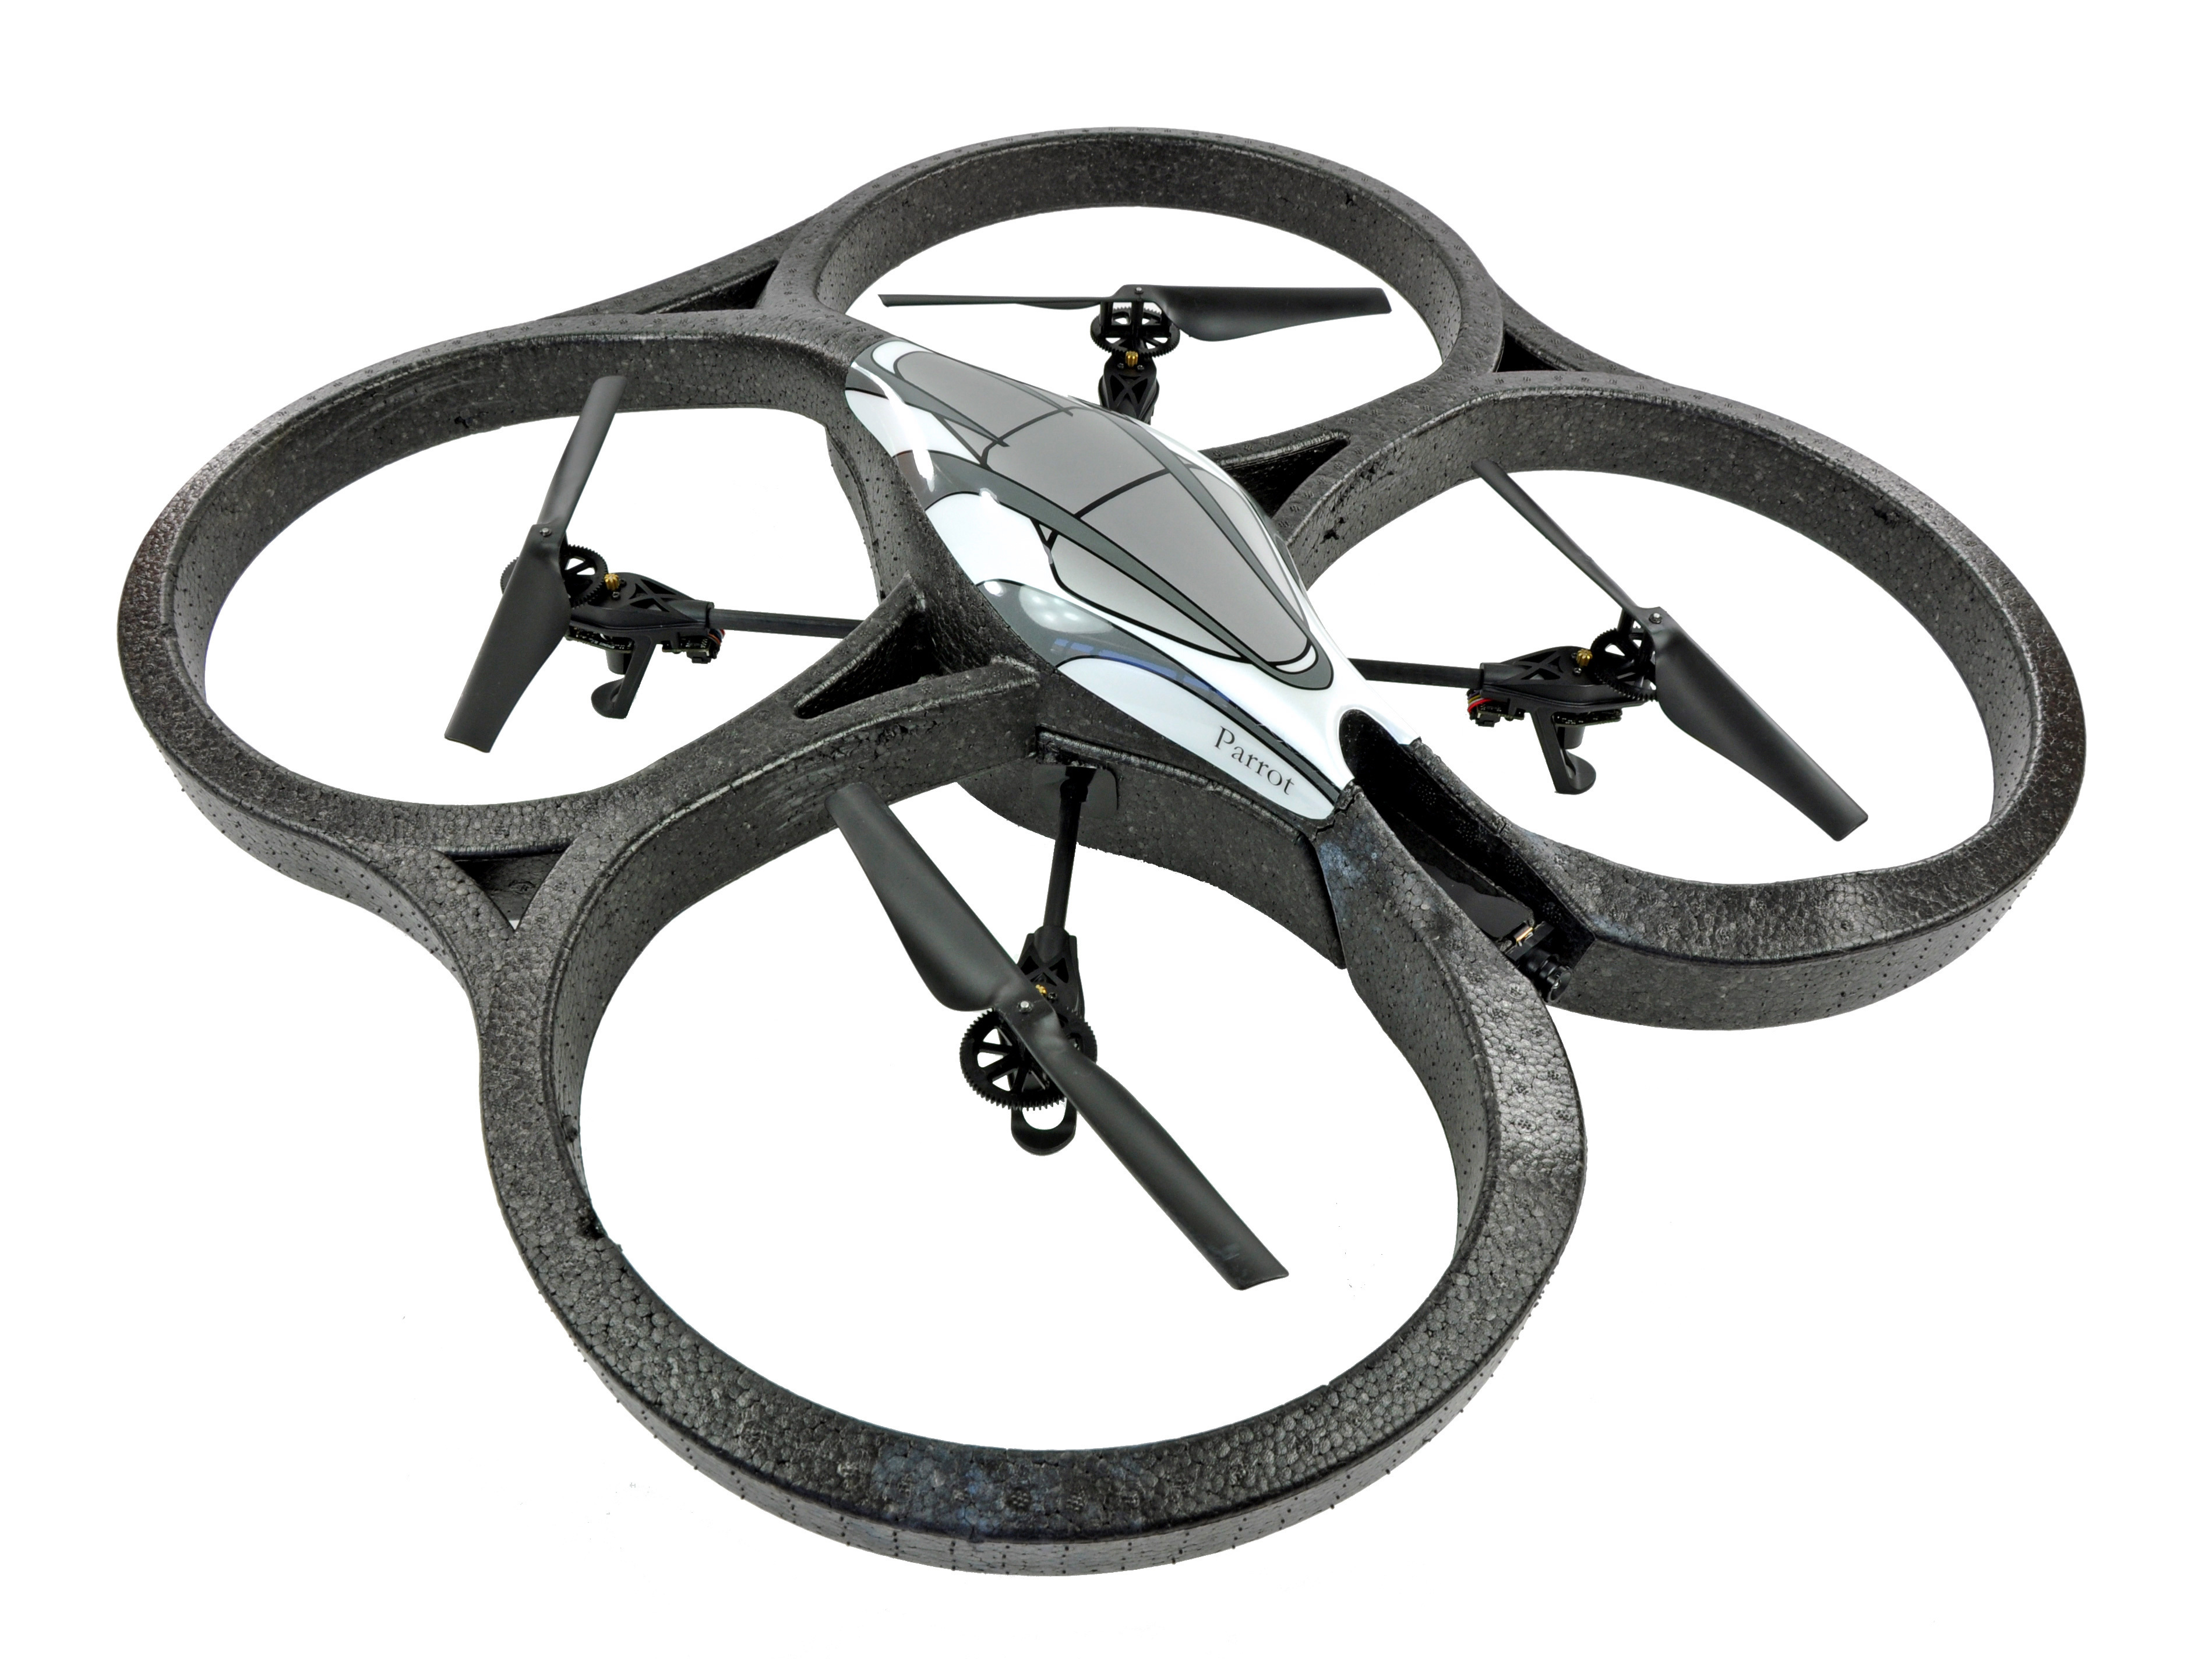
\includegraphics[width=.8\linewidth]{drone.jpg}
\end{subfigure}
\end{figure}

\paragraph {} The controlling application is written in JavaScript and tested
in a notebook and an ARM board (that has the added advantage of being light
enough to be carried by the drone, enabling long range autonomous flights)
\begin{figure}[hbtp]
  \centering
\begin{subfigure}{.99\textwidth}
  \centering
  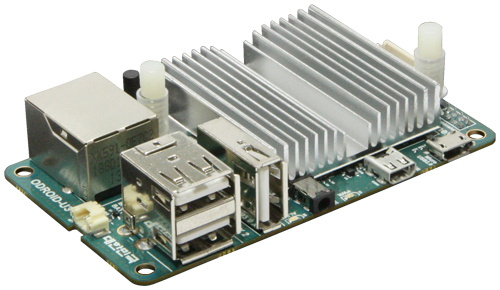
\includegraphics[width=.8\linewidth]{odroid.jpg}
\end{subfigure}
\end{figure}

\section{The solution}
\paragraph {} The solution is divided in 2 independent modules, a controlling
application that communicates with the drone and the pattern matcher that
finds the pattern and gives commands to the controller, this applications
communicate through a web interface and do not need to be hosted in the same
machine.
\paragraph {} The controlling application is based in a NodeJS library that
handles the low level communication, it exports a series of URLs that correspond
to various functions of the drone.\\
The API is very high level and abstracts away details related to flight (for
example, instead of dealing with the default coordinate system for aircraft's,
[roll, pitch, yaw], which would require a very fine tuned propeller control
(incidentally making quad-copters almost impossible to flight without computer
aid). Commands are given based on the drone current coordinate system, in a
[X,Y,Z] frame centered in the middle of the drone, with the X axis pointing
towards the camera, the Z axis being the altitude and the Y axis from left to
right.\\
The camera being positioned along the X axis is a great feature in controlling
the drone both in First Person View flight and in controlling using images, as
it permits a direct association between the position of objects in the image and
the commands needed to move then to the center of the image (for example, if in
the 640x360 image the point is in 100,300, we know the object is at left and
below the drone) (0,0 being the top left corner and 640,360 the bottom right)
%Add a photo here, with the coordinates anotated
\paragraph {} The functions available in the API are:
\begin{itemize}
\item takeoff\\Start propellers, and rise to about 1m.
\item land\\Stop any movement, levels the drone and descend until close the
ground, then stop propellers.
\item up ([speed, optional, default 0.5],[time, optional, default 500ms])\\
This command makes the drone climb, increasing Z
\item down ([speed, optional, default 0.5],[time, optional, default 500ms])\\
This command makes the drone descend, decreasing Z
\item front ([speed, optional, default 0.5],[time, optional, default 500ms])\\
This command makes the drone lean in its front, making it move forward,
increasing X.
\item back ([speed, optional, default 0.5],[time, optional, default 500ms])\\
This command makes the drone lean in its back, making it move backward,
decreasing X.
\item left ([speed, optional, default 0.5],[time, optional, default 500ms])\\
This command makes the drone lean on its lean on its left side, making it move
to the left, decreasing Y
\item right ([speed, optional, default 0.5],[time, optional, default 500ms])\\
This command makes the drone lean on its lean on its right side, making it move
to the right, increasing Y
\item rotatel ([speed, optional, default 0.5],[time, optional, default 500ms])\\
This command makes the drone rotate counter-clockwise over Z
\item rotater ([speed, optional, default 0.5],[time, optional, default 500ms])\\
This command makes the drone rotate clockwise over Z
\item stop\\
This command levels the drone immediately
\item flip\\
This command performs a flip, do not execute it near the ground, walls or other
structures
\item img.jpg\\
This command returns a jpg snapshot from the drone
\end{itemize}
\paragraph {} The functions are exported by a Web API available by accessing
the URL IP:8002/functionName. Parameters can be passed by GET or POST,
eg: 127.0.0.1:8002/up?speed=0.8\&time=100
\paragraph{} The speed parameter determines how much the drone will unbalance
itself, being 1 the maximum supported value and 0 not tilting at all. Higher
values lead to faster movements. The time parameter defines how long until the
drone stabilizes itself again.

\paragraph {} More then one application can access this API at a time, there are
no security features implemented for now, but it would not be hard to add an
authorization token.

\paragraph {} The pattern matching application is composed of:
\begin{itemize}
  \item A SURF detector from OpenCV\\
\begin{verbatim}
	img = image from drone camera, already binarized and filtered
	template = image of the template
	surf = cv2.SURF(400) #400 is an adequate threshold according to tests
	skp, sd = surf.detectAndCompute(img,None)
	#skp contains the image key-points, sd contains the descriptors
	tkp, td = surf.detectAndCompute(template,None)
\end{verbatim}
SURF is responsible for finding key-points in an image. A key-point is a point
in the image with some robust feature. A robust feature is a detail of an image
that can be detected even if its scaled, rotated, or slightly deformed.\\
The images bellow have their key-points marked, the first one has a red cross
marking the position of the pattern in the image.
\begin{figure}[hbtp]
  \centering
SURF
\begin{subfigure}{1.00\textwidth}
  \centering
  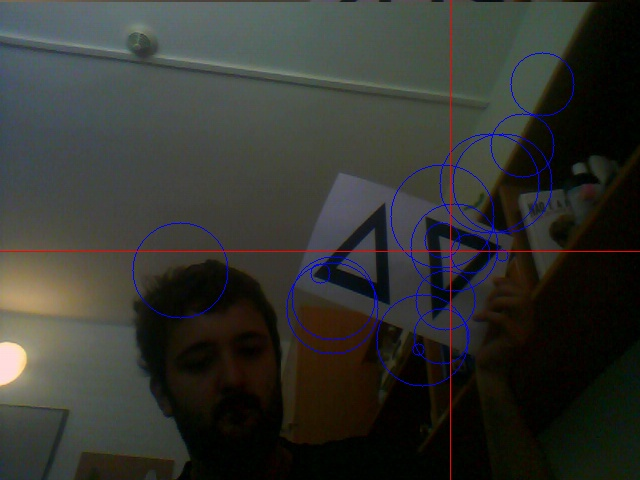
\includegraphics[width=1.0\linewidth]{image_marked.jpg}
  The size of the circle indicates the confidence in the match, this circles are
already filtered.
\end{subfigure}
\begin{subfigure}{1.00\textwidth}
  \centering
  
\includegraphics[width=1.0\linewidth]{template_marked.jpg}
  The template is a pair of triangles as well marked corners are easy to match.
\end{subfigure}
\end{figure}
\newpage
\item A FLANN matcher from OpenCV\\
FLANN is a smart algorithm to find matches in a set of data points, it was used
in place of an exhaustive search because, despite not being as accurate, it is
good enough and a lot faster, enabling the algorithm to run in a cheap ARM board
with low power requirements.\\
This piece of code below runs OpenCV FLANN on both key-point sets and find the
best matches
\begin{verbatim}
    flann_params = dict(algorithm=1, trees=4)
    flann = cv2.flann_Index(sd, flann_params)
    idx, dist = flann.knnSearch(td, 1, params={})
    del flann

    dist = dist[:,0]/2500.0
    dist = dist.reshape(-1,).tolist()
    idx = idx.reshape(-1).tolist()
    indices = range(len(dist))
    indices.sort(key=lambda i: dist[i])
    dist = [dist[i] for i in indices]
    idx = [idx[i] for i in indices]
    skp_final = []
    for i, dis in itertools.izip(idx, dist):
        if dis < distance:
            skp_final.append(skp[i])

    flann = cv2.flann_Index(td, flann_params)
    idx, dist = flann.knnSearch(sd, 1, params={})
    del flann

    dist = dist[:,0]/2500.0
    dist = dist.reshape(-1,).tolist()
    idx = idx.reshape(-1).tolist()
    indices = range(len(dist))
    indices.sort(key=lambda i: dist[i])
    dist = [dist[i] for i in indices]
    idx = [idx[i] for i in indices]
    tkp_final = []
    for i, dis in itertools.izip(idx, dist):
        if dis < distance:
            tkp_final.append(tkp[i])

    return skp_final, tkp_final


\end{verbatim}
\begin{figure}[hbtp]
  \centering
FLANN
\begin{subfigure}{1.00\textwidth}
  \centering
  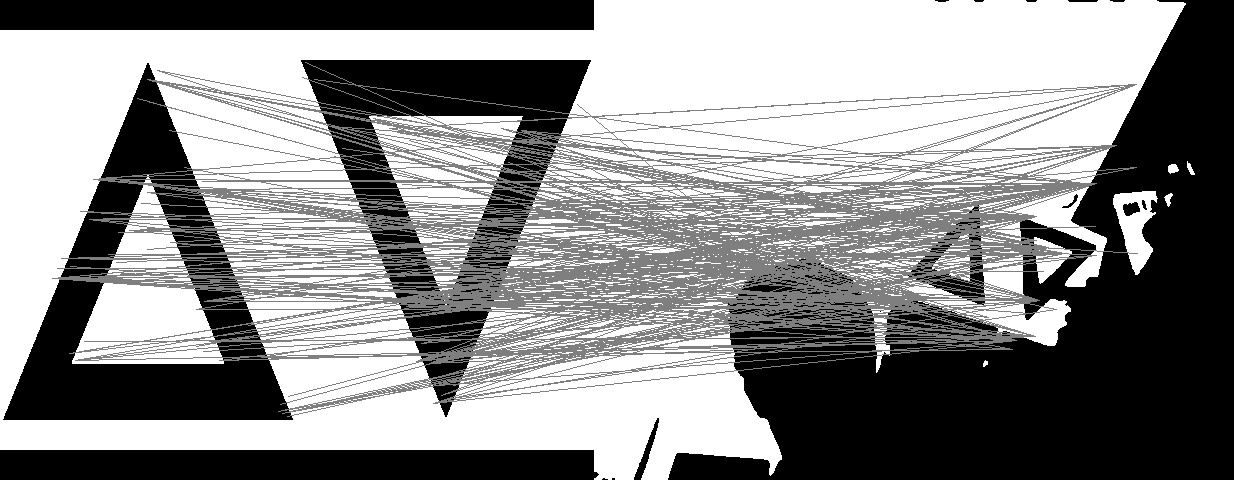
\includegraphics[width=1.00\linewidth]{matches.jpg}
\end{subfigure}
\end{figure}
As seem in the image, SURF was applied to a binarized image, this was done as it
reduce problems related to illumination.

  \item A filter: It is possible to see many imperfect matches, they are
filtered out by iteractively removing the points farther away from the gravity
center of the set.

  \item A decision algorithm: A simple algorithm to decide in witch direction
the drone should move based on where the pattern is found (for up, down, left
and right), and the size it appears to have (for front and back), at this
iteration of the project the drone is set to move at only 30\% of its speed
and move for 0.5s at a time.\\
The drone stays still when no pattern is detected, in a future iteration it
could be useful to have the drone rotating or flying in circles, as it would
increase the chance it would come across the pattern changing the point of
view.
\end{itemize}
\paragraph{} The application process a image in less then 50ms, but the rate is
limited to 2Hz as its more then enough to control the drone and leave a lot of
room for both improvements in this application and other applications running in
the controller (as a flight stabilizer or a GPS tracker).

\section{The Results}
\paragraph {} In the following 3 pages a log of a test flight is included, it
consists of the output from the pattern matcher, to be read as:
\begin{itemize}
\item Date
\item Position (x,y) of the pattern and the geometry of the image
\item Log of commands executed
\end{itemize}
\paragraph{} At this iteration the pattern matcher was not modulating the speed
and time for each function. It was also not commanding the drone to go front or
back as this section of the code is still not reliable enough for pure
autonomous flight.
\newpage
\begin{verbatim}
Wed May 13 14:18:04 CEST 2015
(371, 268, (640,360))
goright
godown
Wed May 13 14:18:05 CEST 2015
(367, 268, (640,360))
godown
Wed May 13 14:18:09 CEST 2015
(322, 205, (640,360))
Wed May 13 14:18:11 CEST 2015
(459, 251, (640,360))
goright
godown
Wed May 13 14:18:13 CEST 2015
(292, 303, (640,360))
godown
Wed May 13 14:18:14 CEST 2015
(456, 262, (640,360))
goright
godown
Wed May 13 14:18:14 CEST 2015
(352, 192, (640,360))
Wed May 13 14:18:15 CEST 2015
(429, 145, (640,360))
goright
Wed May 13 14:18:16 CEST 2015
(468, 115, (640,360))
goright
goup
Wed May 13 14:18:16 CEST 2015
(404, 125, (640,360))
goright
goup
Wed May 13 14:18:17 CEST 2015
(434, 118, (640,360))
goright
goup
Wed May 13 14:18:19 CEST 2015
(412, 133, (640,360))
goright
Wed May 13 14:18:19 CEST 2015
(441, 180, (640,360))
goright
Wed May 13 14:18:20 CEST 2015
(418, 274, (640,360))
goright
godown
Wed May 13 14:18:21 CEST 2015
(425, 217, (640,360))
goright
Wed May 13 14:18:21 CEST 2015
(411, 232, (640,360))
goright
godown
Wed May 13 14:18:22 CEST 2015
(428, 151, (640,360))
goright
Wed May 13 14:18:23 CEST 2015
(408, 183, (640,360))
goright
Wed May 13 14:18:24 CEST 2015
(423, 136, (640,360))
goright
Wed May 13 14:18:25 CEST 2015
(412, 133, (640,360))
(403, 78, (640,360))
goright
goup
Wed May 13 14:18:26 CEST 2015
(367, 81, (640,360))
goup
Wed May 13 14:18:28 CEST 2015
(416, 58, (640,360))
goright
goup
Wed May 13 14:18:29 CEST 2015
(398, 68, (640,360))
goright
goup
Wed May 13 14:18:31 CEST 2015
(406, 58, (640,360))
goright
goup
Wed May 13 14:18:33 CEST 2015
(297, 74, (640,360))
goup
Wed May 13 14:18:33 CEST 2015
(273, 38, (640,360))
goup
Wed May 13 14:18:35 CEST 2015
(312, 52, (640,360))
goup
Wed May 13 14:18:35 CEST 2015
(310, 51, (640,360))
goup
Wed May 13 14:18:36 CEST 2015
(345, 141, (640,360))
Wed May 13 14:18:37 CEST 2015
(422, 167, (640,360))
goright
Wed May 13 14:18:37 CEST 2015
(472, 171, (640,360))
goright
Wed May 13 14:18:38 CEST 2015
(524, 149, (640,360))
goright
Wed May 13 14:18:39 CEST 2015
(523, 200, (640,360))
goright
\end{verbatim}
\paragraph{} As seen in the logs the drone correctly reacts to the commands
sent, further advances need to be made in modulating the force of the response
based in the position and distance of the target pattern.
\begin{figure}[hbtp]
  \centering
\begin{subfigure}{.99\textwidth}
  \centering
  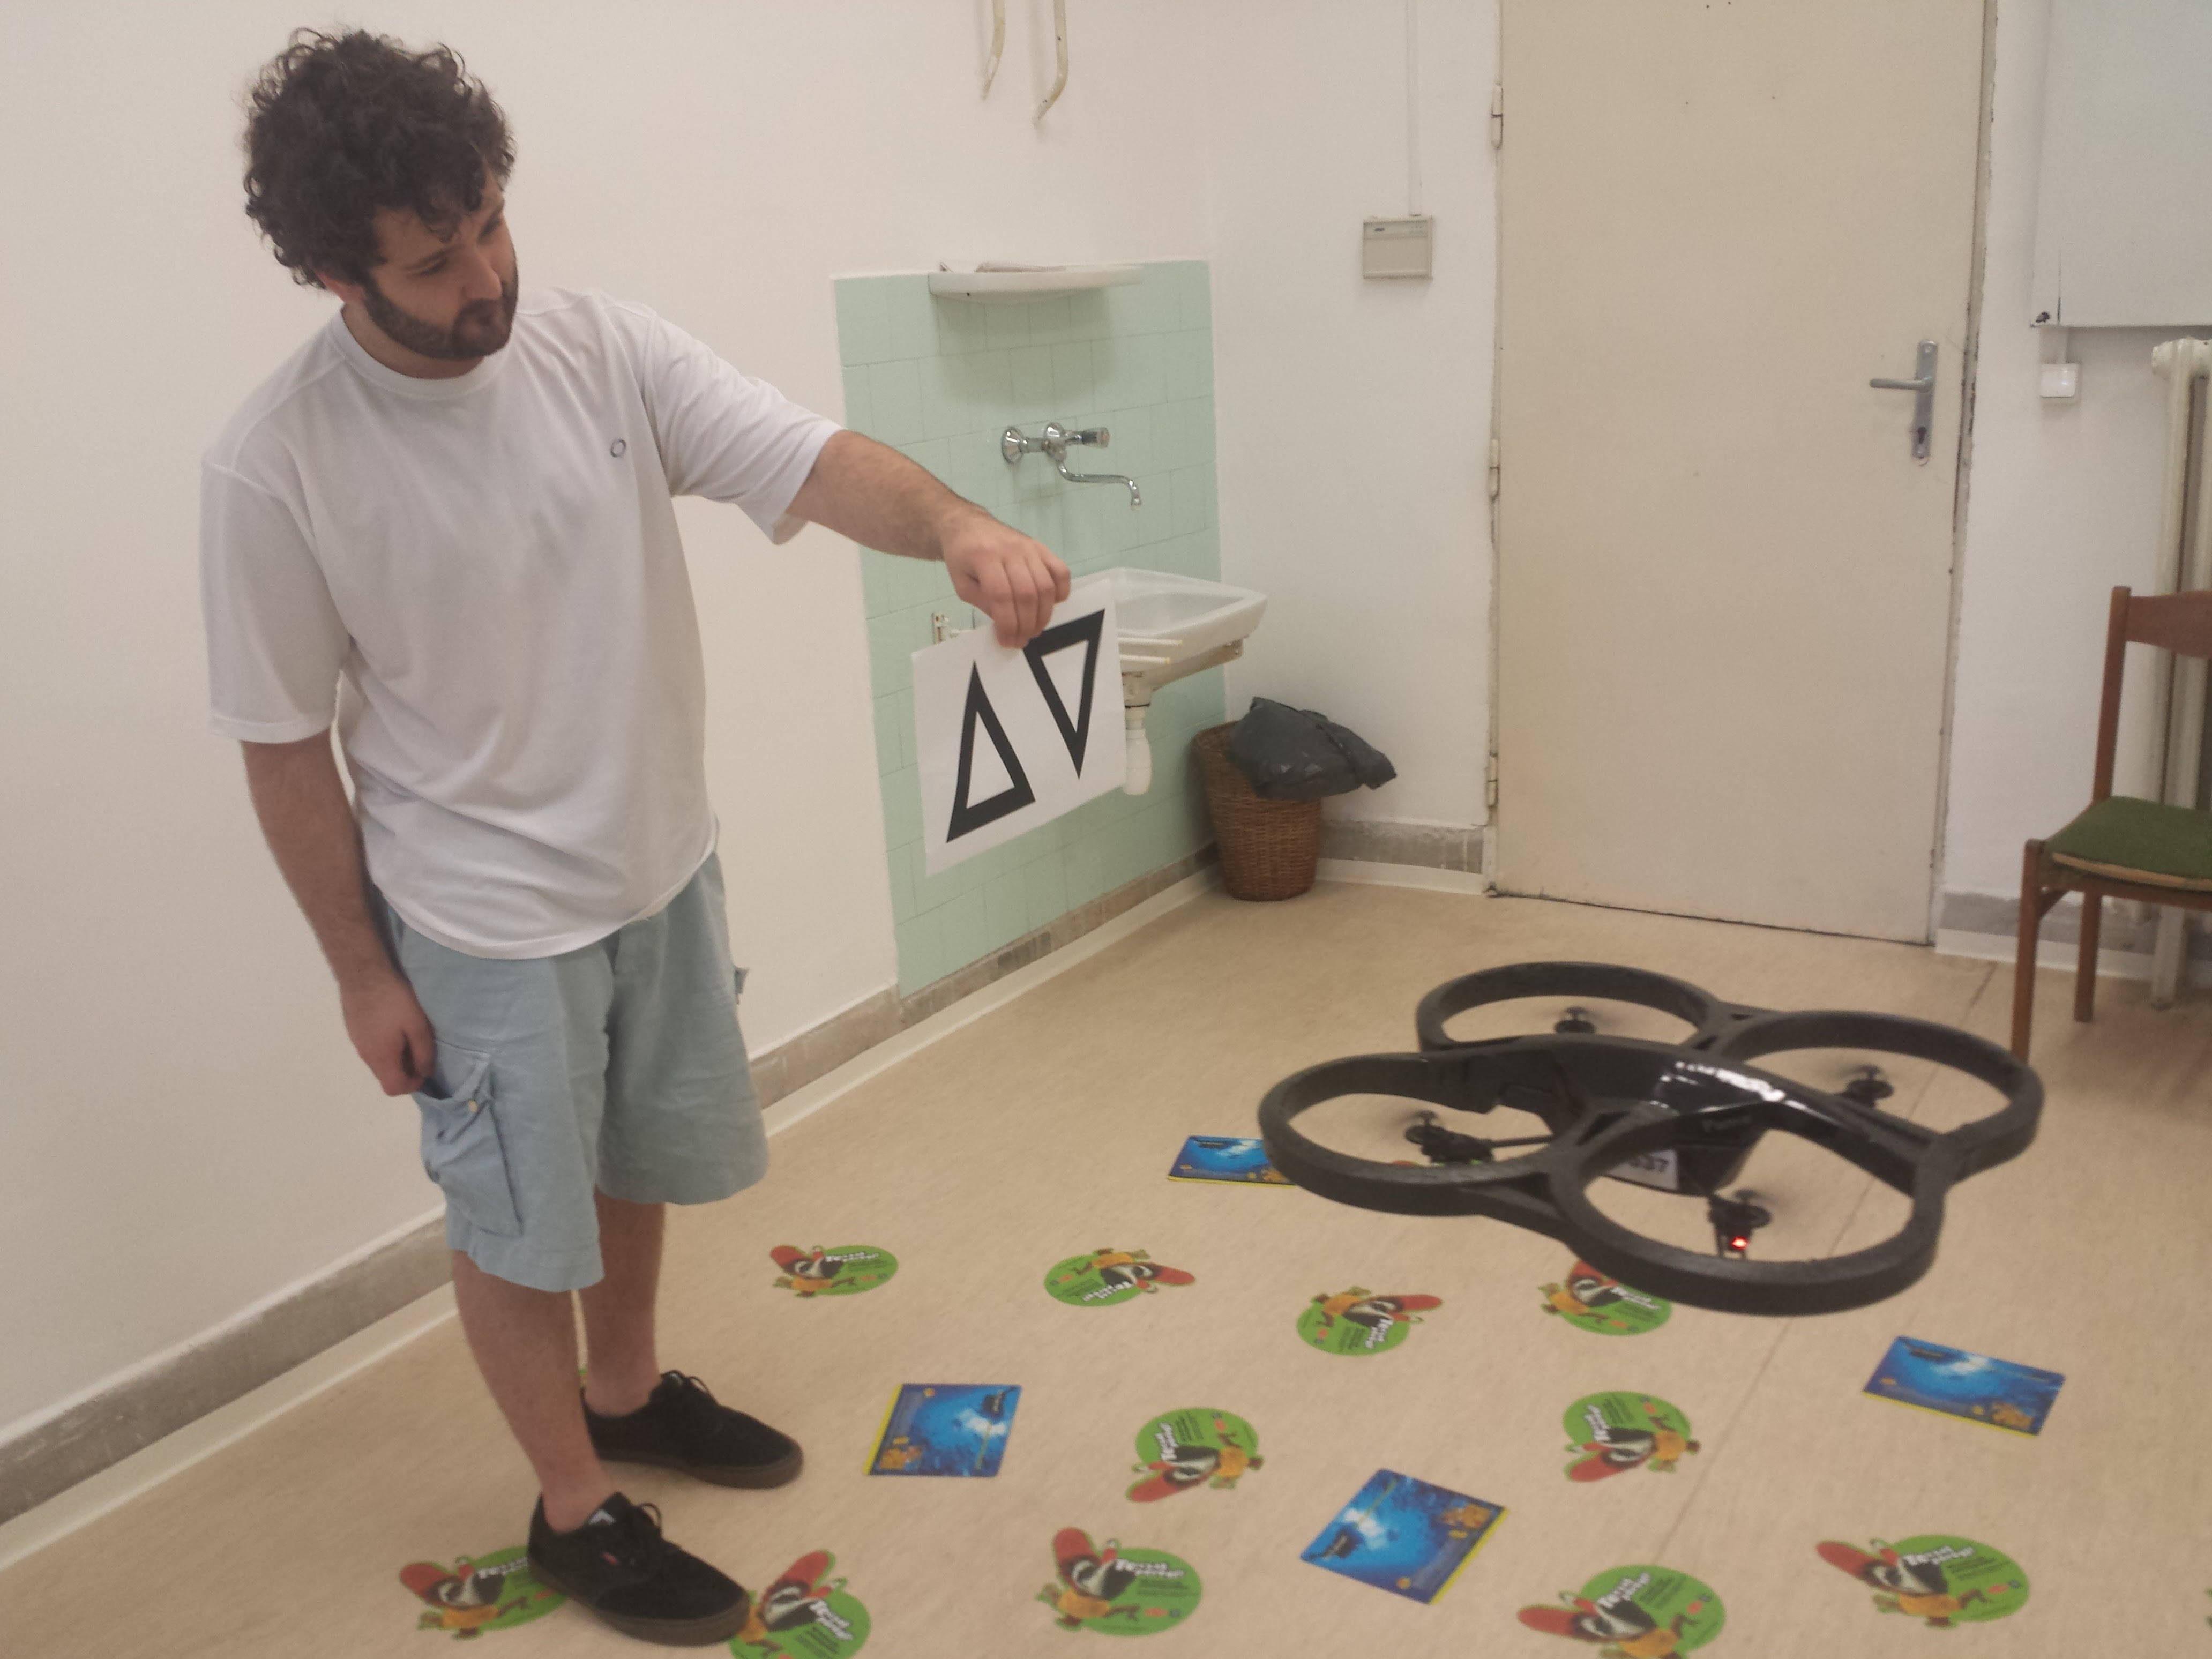
\includegraphics[width=1\linewidth]{tracking.jpg}
Example of the drone following a pattern
\end{subfigure}
\end{figure}


\end{document}
